\let\negmpace\undefined
\let\negthickspace\undefined
\documentclass[journal]{IEEEtran}
\usepackage[a5paper, margin=10mm, onecolumn]{geometry}
%\usepackage{lmodern} % Ensure lmodern is loaded for pdflatex
\usepackage{tfrupee} % Include tfrupee package
\setlength{\headheight}{1cm} % Set the height of the header box
\setlength{\headsep}{0mm}     % Set the distance between the header box and the top of the text
\usepackage{xparse}
\usepackage{gvv-book}
\usepackage{gvv}
\usepackage{cite}
\usepackage{amsmath,amssymb,amsfonts,amsthm}
\usepackage{algorithmic}
\usepackage{graphicx}
\usepackage{textcomp}
\usepackage{xcolor}
\usepackage{txfonts}
\usepackage{listings}
\usepackage{enumitem}
\usepackage{mathtools}
\usepackage{gensymb}
\usepackage{comment}
\usepackage[breaklinks=true]{hyperref}
\usepackage{tkz-euclide} 
\usepackage{listings}
% \usepackage{gvv}                                        
\def\inputGnumericTable{}                                 
\usepackage[latin1]{inputenc}                                
\usepackage{color}                                            
\usepackage{array}                                            
\usepackage{longtable}                                       
\usepackage{calc}                                             
\usepackage{multirow}                                         
\usepackage{hhline}                                           
\usepackage{ifthen}                                           
\usepackage{lscape}
\renewcommand{\thefigure}{\theenumi}
\renewcommand{\thetable}{\theenumi}
\setlength{\intextsep}{10pt} % Space between text and floats
\numberwithin{equation}{enumi}
\numberwithin{figure}{enumi}
\renewcommand{\thetable}{\theenumi}
\begin{document}
\bibliographystyle{IEEEtran}
\title{Question-8.2.1}
\author{EE24BTECH11038 - MALAKALA BALA SUBRAHMANYA ARAVIND}
% \maketitle
% \newpage
% \bigskip
{\let\newpage\relax\maketitle}
\textbf{Question}:
Find the area of the circle $4x^2+4y^2=9$, which is interior to the parabola $x^2=4y$\\
\solution \\

\noindent \textbf{Trapezoidal rule:} It is a numerical method for approximating the definite integral of a function. The classic definition is as follows:\\
Given a function $f\brak{x}$ that is continuous in the interval $\sbrak{a,b}$, the trapezoidal rule approximates the integral by dividing the interval $\sbrak{a,b}$ into n sub intervals of equal width h=$\frac{b-a}{n}$. The x-values at the sub interval boundaries are: 
\begin{align}
    x_0=a,x_1=a+h,x_2=a+2h,\cdots,x_n=b.
\end{align}
The trapezoidal rule then computes the integral as
\begin{align}
    \int_a^b f\brak{x}\,\,dx \approx \frac{h}{2}\brak{f\brak{x_0}+2f\brak{x_1}+2f\brak{x_2}+\cdots +2f\brak{x_{n-1}}+f\brak{x_{n}}}
\end{align}
First we need to calculate the point of intersections of the two given curves
\begin{align}
    y&=\frac{x^2}{4}\\
    x^2+y^2&=\frac{9}{4}\\
    x^2+\frac{x^4}{16}&=\frac{9}{4}\\
    16x^2+x^4&=36
\end{align}
on solving the equation we get x values as $\sqrt{2}$ and $-\sqrt{2}$\\
so the points of intersection of both curves are $\brak{\pm \sqrt{2},\frac{1}{2}}$\\
The interval $\sbrak{-\sqrt{2},\sqrt{2}}$ is divided into 1000 sub intervals each of width h=$\frac{2\sqrt{2}}{1000}$ then the points in the interval can be written as 
\begin{align}
    x_i=-\sqrt{2}+i\cdot h\\
    \text{Area} \approx \frac{h}{2}\sbrak{f\brak{x_0}+2\sum_{i=1}^{n-1} f\brak{x_i}+f\brak{x_n}}\\
    f\brak{x_i}=\sqrt{\frac{9}{4}-x_i^2}-\frac{x_i^2}{4}
\end{align}
Using a c code to find the area using trapezoidal rule i got the area as
\begin{align}
    A \approx 3.0054
\end{align}
If the area is calculated directly using integration method the area would be around 3.063 which  is so close to the one we found using trapezoidal rule 
\begin{figure}
	\centering
	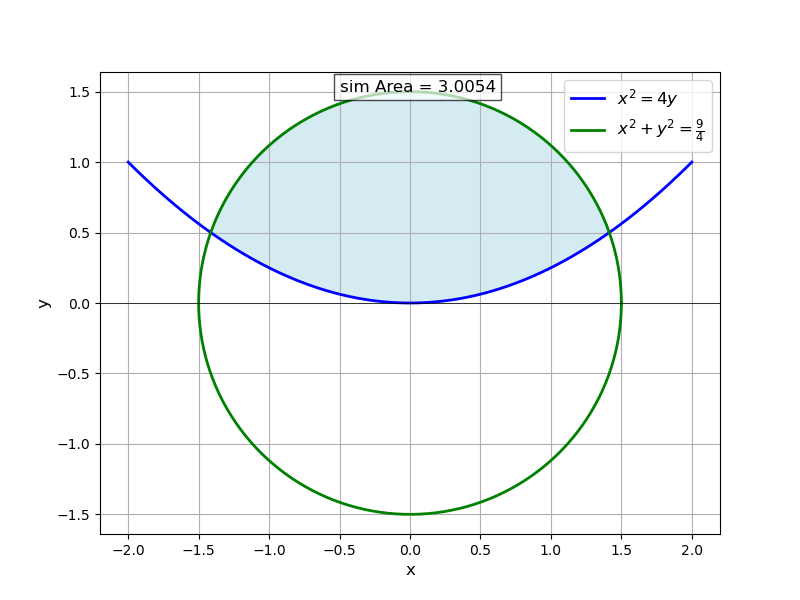
\includegraphics[width=\columnwidth]{figs/Figure_1.png}
	\label{stemplot}
\end{figure}	

\end{document}
